\chapter{Overlapping Reconstructions}
\label{ch:overlapping}

\section{Purpose}
\label{sec:overlapping-purpose}

Frazier et al. demonstrate that the sona of a given interrogation pulse is significantly longer than the pulse that generated it~\cite{nltr-wave-chaotic}. This stands to reason, given that the sona represents reflections of the initial pulse shifted in time by differing path lengths.

The reverse is also true: A time reversed sona will generate a reconstruction that is significantly shorter than it in time. This trait imposes a limitation on the ability of time reversal to transmit power. However, transmitting multiple sonas at once from the same antenna is possible--copying and shifting the signal in time can allow more data to be sent in one transmission cycle. This will in turn result in multiple transmitted reconstructions, and improved power transmission.

A concern with the above method is whether or not it would result in lost information. Sonas are sinusoidal signals--if overlaid, they will interfere constructively and destructively. Destructive interference may result in the ``deletion'' of transmission paths, reducing the fidelity of the created reconstructions.

\section{Methodology}
\label{sec:overlapping-meth}

This test sought to test the practicality of overlapping sonas as a method of transmitting power. This experiment was done using the linear time reversal setup described in Section~\ref{sec:linear-methodology}. A sona was generated connecting a given starting and ending point. To prove that the sona could converge on the target, it was time reversed without any further manipulation, and the reconstruction was measured.

Once the efficacy of the sona was established, overlapping sonas were created. overlapping sonas were created by copying and evenly spacing the original sona in time across the broadcast window, or the span of time over which the signal was broadcast. Figure~\ref{fig:overlapping-sonas} gives an example of sonas overlapping in this way. The overlapping sonas were time reversed and broadcast through the linear system in the same manner as before, which resulted in the reconstructions in Figure~\ref{fig:overlapping-recons}.

\begin{figure}[t]
\centering
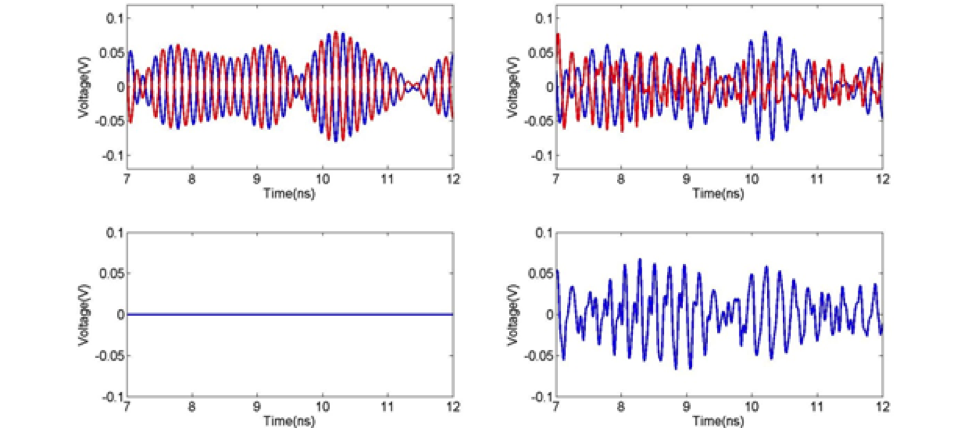
\includegraphics[width=0.85\textwidth]{overlapping/sonas}
\caption[Overlapping sonas]{Overlapping sonas with a spacing of 7.5 $\mu$s.}
\label{fig:overlapping-sonas}
\end{figure}

\begin{figure}[t]
\centering
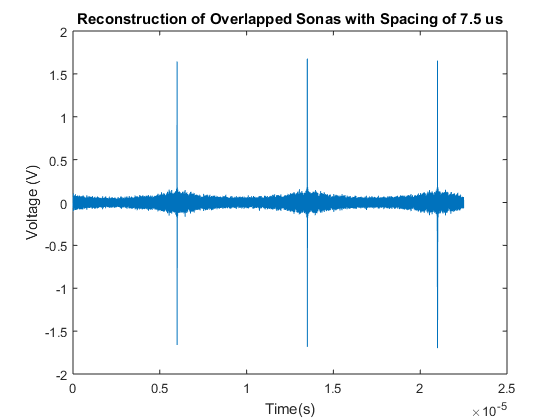
\includegraphics[width=0.85\textwidth]{overlapping/recons}
\caption[Overlapping reconstructions]{Reconstructions resulting from the sonas in~\ref{fig:overlapping-sonas}.}
\label{fig:overlapping-recons}
\end{figure}

\begin{figure}[t]
\centering
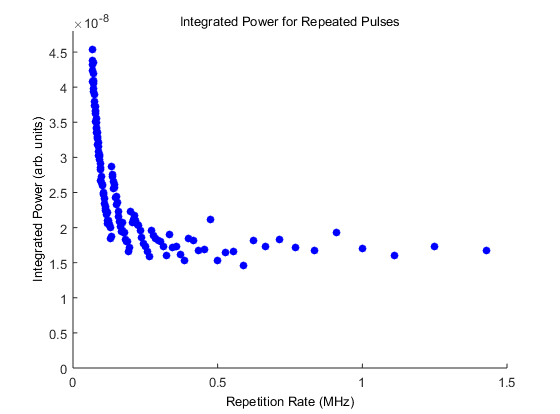
\includegraphics[width=0.85\textwidth]{overlapping/power}
\caption[Power from overlapping reconstructions]{Integrated power from overlapping reconstructions.}
\label{fig:overlapping-power}
\end{figure}

\section{Results}
\label{sec:overlapping-results}

Sonas were tested with offsets between 0.1~$\mu$s and 15~$\mu$s, by increments of 0.1~$\mu$s. The average peak to peak voltages of reconstructions created with these sonas are plotted in Figure~\ref{fig:overlapping-power}. Increasing the number of sonas should, logically, increase the amount of power transmitted in a given time frame. However, the trend observed in Figure~\ref{fig:overlapping-power} is much more complex than this. We believe these results to be a result of the internal power settings of the PSG: it attempts to level the total amount of power leaving (and has only so much to give per cycle), which results in the discontinuities when mechanically switching source components throughout the sweep.


\section{Discussion}
\label{sec:overlapping-discussion}

We hypothesized that overlapping reconsturctions by overlaying sonas could result in more effective power transmitted per duty cycle. Our experiments seemed to support this in that the number of reconstructions in the cycle could be increased while maintaining their characteristic shape. However, our lab equipment attempted to scale each arbitrary waveform we broadcast to the same total output power. This prevented us from definitively finding a relationship between the number of reconstructions and the power received by the target.
